\documentclass[../portafolio.tex]{subfiles}

\begin{document}

% En esta sección, explique en detalle los siguientes aspectos:
% - Fecha de realización de la actividad
% - Título de la actividad (dentro de \section)
% - Un párrafo explicando cuál es el objetivo de la actividad
% - Nombre de personas con quien trabajó en la actividad
% - Una selección de evidencias de que usted hizo esta actividad (imágenes, códigos, respuestas a un problema teórico, etc.)
% - Una conclusión breve (qué aprendió con la actividad, qué no entendió, qué faltó trabajar, qué recomienda para futuras sesiones)

% Numero máximo de palabras en esta sección: 1000 palabras.

%%%%%%%%%%%%%%%%%%%%%%%%%%%%%%%%%%%%%%%%%%%%%%%%%%%%%%%%%%%%%%%%%%%%%%%%%%%%%%%%
\section{Fractal de Newton} 

\hfill \textbf{Fecha de la actividad:} 28 de septiembre de 2022

\medskip

%---------------------------------------------------------------------------------
% Introducción/objetivos de la actividad
En esta actividad, graficaremos el fractal de Newton~\cite{ref:newton-fractal} para el polinomio
$f(z)=z^3-1$, el cual tiene 3 ceros o raices complejas de módulo
unitario. El fractal se construye resolviendo $f(z)=0$ usando el
método de Newton-Raphson:
\begin{align}
  \label{eq:newton-raphson}
  z_{i+1}
  &= z_{i} - \frac{f(z_i)}{f'(z_i)} \,,
  \\
  &= z_{i} - \frac{1}{3} \left( z - 1/z^2\right) \,.
\end{align}
%  

El método de Newton-Raphson solo converge a una de las tres soluciones
de $f(z)=0$ dependiendo de la semilla inicial $z_0$. Por ello, el
objetivo es estudiar cómo converge el método para distintos valores de
$z_0$. Para cada $z_0$, graficaremos ese punto en el plano complejo y
lo pintaremos de acuerdo a la fase de la solución a la que converge el
método.


%---------------------------------------------------------------------------------
% Selección de evidencias
El método de Newton-Raphson~\cite{ref:newton-raphson} se codifica en el código~\ref{cod:newton}.
\begin{listing}
  \begin{pythoncode}
def newton(semilla, N=3, maxerr=1e-3):
    z   = semilla
    err = maxerr+1
    it = 0
    while np.abs(err)>maxerr:
        err = (z-z**(1-N)) / N
        z = z - err
        it = it + 1

    return z, it
\end{pythoncode}
\caption{Método de Newton para encontrar los ceros de $f(z)=z^3-1$.}
\label{cod:newton}
\end{listing}


Luego, escogemos varias semillas $z_0$ en el plano complejo dentro de la
región $x_\text{min}<\text{Re}(z)<x_\text{max}$ y
$y_\text{min}<\text{Im}(z)<y_\text{max}$, y usamos el método de
Newton-Raphson para cada una de estas semillas.
\begin{pythoncode}
  sol = [[ newton(semilla=complex(xi,yi), N=3)
           for yi in linspace(ymin, ymax, Ny)
         ]
         for xi in linspace(xmin, xmax, Nx)]
\end{pythoncode}

Cada punto $z_0$ del plano complejo en la región mostrada se utiliza como semilla del método de Newton-Raphson para encontrar los ceros de $f(z)$. Si el método converge a $z=e^{i\phi}$, el punto $z_0$ es pintado de acuerdo al valor de la fase $\phi$. En este caso, los posibles valores de la fase son $\phi=\{0,2\pi/3,5\pi/3\}$.

\begin{figure}[ht!]
  \centering
  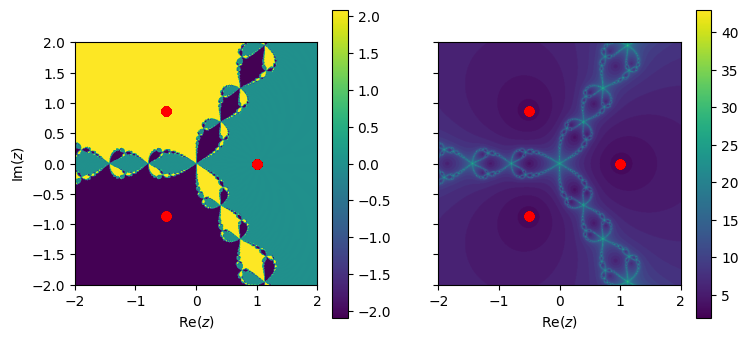
\includegraphics[width=\textwidth]{newton-fractal}
  \caption{Fractal de Newton asociado a la ecuación $f(z)=z^3-1$. (izquierda) La barra de colores representa la fase $\phi$ de los ceros $z=e^{i\phi}$ de $f(z)$ a los que converge el método de Newton-Raphson. (derecha) La barra de colores representa el número de iteraciones que requiere el método de Newton-Raphson para converger a uno de los ceros de $f(z)$. }
  \label{fig:In_series_trapz}
\end{figure}
  

  
\end{document}
